\documentclass[11pt,titlepage,openright]{book}
\usepackage[utf8]{inputenc}
\usepackage[T1]{fontenc}
\usepackage[british]{babel}
\usepackage{graphicx}
\usepackage[dvipsnames]{xcolor}
\usepackage[sb]{libertine}
\usepackage[scale=0.9]{inconsolata}



\usepackage[sf]{titlesec}
\usepackage[numbers]{natbib}
%\usepackage[export]{adjustbox}

\usepackage{
  marginnote, % Improved margin notes
  environ,
  ragged2e,   % Justified text in the margin notes
  url,        % For typesetting URLs
  listings,   % Code formatting
  hyperref,   % Links in PDF from TOC, refs, etc.
  lipsum,
  booktabs,
  changepage,
  float,
  dingbat
}
\renewcommand{\bfdefault}{bx}
\DeclareTextFontCommand\textsb{\libertineSB}

\usepackage[capitalise]{cleveref}
\Crefname{section}{\S}{\S\S}

\usepackage{enumitem}   % Improved lists 
% \setlist{noitemsep} % To make all lists compact
\setlist[itemize]{itemsep=0pt}
\setlist[itemize,1]{label=--}
\setlist[itemize,2]{label=\ensuremath{\triangleright}}
\setlist[itemize,3]{label=\RED{AVOID}}
% Description lists to use semibold labels
\setlist[description]{font=\libertineSB}

\usepackage[twoside,labelfont=sf]{caption}

\usepackage{float}

\captionsetup{justification=raggedright,singlelinecheck=false}

\newcommand\myhrulefill[1]{\leavevmode\leaders\hrule height#1\hfill\kern0pt}
\DeclareCaptionFormat{FigFormat}{{\color{black}\myhrulefill{0.5pt}}\\#1#2#3}
\captionsetup[figure]{format=FigFormat}
\captionsetup[table]{format=FigFormat}

\DeclareCaptionFormat{LstFormat}{\textsf{Listing}~\arabic{chapter}.\arabic{listing}:#2#3}
\floatstyle{ruled}
\newfloat{listing}{thp}{lol}[chapter]
\floatname{listing}{Listing}
\captionsetup[listing]{format=LstFormat}

\NewEnviron{MarginNote}[1][0mm]{\marginnote{\footnotesize\justifying\BODY}[#1]}
\newcommand{\Footnote}[2][0mm]{\footnotemark\marginnote{\footnotesize$^{\arabic{footnote})}$~#2}[#1]}

\renewenvironment{figure*}[1][]{%
  \begin{figure}[#1]%
    % This feature is deprecated for now
    % \checkoddpage%
    % \ifoddpage%
    %   \begin{adjustwidth}{0cm}{-45mm}%%
    % \else%
    %   \begin{adjustwidth}{-45mm}{0cm}%%
    % \fi%
    }{%
    % \end{adjustwidth}%
  \end{figure}}

\renewenvironment{table*}[1][]{%
  \begin{table}[#1]%
    % This feature is deprecated for now
    % \checkoddpage%
    % \ifoddpage%
    %   \begin{adjustwidth}{0cm}{-45mm}%%
    % \else%
    %   \begin{adjustwidth}{-45mm}{0cm}%%
    % \fi%
    }{%
    % \end{adjustwidth}%
  \end{table}}

\renewenvironment{listing*}[1][]{%
  \begin{listing}[#1]%
    % This feature is deprecated for now
    % \checkoddpage%
    % \ifoddpage%
    %   \begin{adjustwidth}{0cm}{-45mm}%%
    % \else%
    %   \begin{adjustwidth}{-45mm}{0cm}%%
    % \fi%
    }{%
    % \end{adjustwidth}%
  \end{listing}}

%% == Code =======================================================
\lstnewenvironment{Code}[1][style=std]{\lstset{#1}}{}
\lstnewenvironment{Code_Numbered}[1][style=std,numbers=left]{\lstset{#1}}{}

\renewcommand{\c}[1]{\lstinline[style=std]@#1@}

\lstset{
  basicstyle=\ttfamily\small,
  keywordstyle=\color{blue}\bfseries,
  commentstyle=\color{gray}\itshape,
  stringstyle=\color{orange},
  showstringspaces=false,
  numbers=left,
  numberstyle=\tiny\color{gray},
  numbersep=8pt,
  frame=single,
  breaklines=true,
  captionpos=b,
}

\lstdefinestyle{std}{
  language=java,
  basicstyle=\small\tt\color{black},
  keywordstyle=\small\tt\bfseries,
  numberstyle=\footnotesize\sf\color{black},
  commentstyle=\small\color{black}\it,
  aboveskip=1ex,
  belowskip=1ex,
  tabsize=2,
  columns=fullflexible,
  xleftmargin=1ex,
  resetmargins=true,
  showstringspaces=false,
  morecomment=[l]{//},
  morecomment=[l]{--},
  morecomment=[s]{/*}{*/},
  escapeinside=@@,
  morekeywords={Frobies},
  moredelim=[is][\textit]{___}{___},
  moredelim=[is][\textbf]{__*}{*__},
  numberbychapter=true
}

\lstdefinelanguage{Scala}{
  keywords={def, val, var, class, object, extends, trait, 
             case, match, if, else, return, import, new,
             true, false, override, sealed, abstract, require},
  otherkeywords={=>, <-, @},
  sensitive=true,
  comment=[l]{//},
  morecomment=[s]{/*}{*/},
  morestring=[b]",
}

\usepackage[activate={true,nocompatibility},final,tracking=true,kerning=true,spacing=true,factor=1100,stretch=10,shrink=10]{microtype}
\usepackage[paper=a4paper,text={13cm,24cm},marginparsep=5mm,marginparwidth=45mm,inner=20mm,twoside]{geometry}

\newcommand{\RED}[1]{\textcolor{red}{#1}}
\newcommand{\ie}{\emph{i.e.,}}
\newcommand{\eg}{\emph{e.g.,}}
\newcommand{\etal}{\emph{et~al.}}

\usepackage{pifont}
\newcommand{\Yes}{\ding{51}}
\newcommand{\No}{\ding{55}}

\renewcommand{\bfdefault}{b}
\clearpage{\pagestyle{empty}\cleardoublepage}

%% You can remove this line if you compile with --synctex=1 (see Makefile)
\synctex=1
\pagestyle{plain}

\begin{document}
\frontmatter
\title{Evaluating Stainless on SV-COMP}
\author{Hadi Saleh}
\date{\today}

\maketitle

\vspace*{3cm}
\section*{Abstract}

\RED{Replace this with the actual abstract. Obviously.}
Suspendisse luctus leo et porta mattis. In semper, nisi et
suscipit iaculis, leo urna laoreet lacus, ut laoreet lorem tellus
eget dui. Vestibulum eu auctor nisi. Morbi pharetra euismod velit
ac mattis. Maecenas tempor vitae augue ut aliquam. Nunc auctor,
nibh at imperdiet finibus, ex leo semper lacus, ac vehicula quam
nisl condimentum leo.


\tableofcontents
\listoffigures
\listoftables

\mainmatter

\chapter{Introduction}
As software becomes increasingly deployed to critical systems in society,
everything from medical devices to vehicles to financial infrastructure. 
As the complexity of such systems advance, 
the cost of undetected defects drastically increases as well.
A major important element of such software then becomes to ensure and
verify that they behave correctly and as expected.  

A common way to ensure this is to have them tested and verified 
to make sure that such software and systems do what they are 
intended to do, therefore making them more reliable and safe to use. 
Traditional testing methods, where a set of inputs gets run through
the program and the outputs get checked against the corresponding 
expected results. While this is still useful, 
it would only demonstrate the presence of defects, 
and not their absence. For programs with large or even infinite 
input ranges, testing them in such a way would be infeasible.

In response to this, formal verification tools
developed to provide mathematical guarantees that a program satisfies
its specifications for \emph{all} valid inputs. An example of such a 
tool is Stainless~\cite{StainlessOriginal}, developed at EPFL for programs written
in the Scala programming language. Stainless is
a deductive verification framework, meaning that it proves 
program correctness from formal specifications using mathematical
logical reasoning. It verifies the programs functional correctness,
termination and absence of runtime errors. 

However, such verifiers aren't guaranteed to be flawless and can 
fail to verify correct programs, timeout, or produce false evaluations.
To adress this issue and benchmark verification tools systematically
, there is an annual verifier benchmark competition
called SV-COMP~\cite{SV-COMP}, which maintains a large amount 
of benchmarks covering a wide range of verification tasks primarly focused
on C and Java verifiers and validators. 
 
Although, Stainless appeared promising in different studies (cite studies), 
it has yet to be evaluated on a large scale benchmark such as SV-COMP.
This project addresses the gap by evaluating Stainless on SV-COMP benchmarks
through translating the benchmark programs used in SV-COMP on Java verifiers, 
to equivalent Scala programs and running Stainless on them. The results 
are then evaluated and compared to the Java verifiers' benchmarks.

\section{Formal Verification}

Formal verification, the underlying concept of 
this project, is the process of 
mathematically proving that a program satisfies a set 
of specifications for all possible inputs. 
On the other hand, testing would only be able to demonstrate 
the presence of bugs on a subset of inputs while formal 
verification provides guarantees that would hold universally. 
This makes formal verification particularly valuable in 
domains where safety is crucial and the cost of 
undetected defects is high.

There are multiple approaches to formal verification. 
\textbf{Model Checking} is the process of 
    exhaustively exploring a program's state space to 
    check whether a property holds or not. 
    However, it can suffer from state space explosion for 
    large programs~\cite{ModelChecking}.
\textbf{Static Analysis} approximates the program's behavior 
    to infer properties without having to execute the actual 
    program, meaning that it trades precision for scalability~\cite{StaticAnalysis}.
\textbf{Deductive Verification}, the approach most
    relevant to this project, requires that the developer 
    annotates the program with some formal specifications to 
    describe the expected behaviour of the program, such 
    as preconditions and postconditions on functions, loop invariants, 
    and assertions. The verifier then uses logical reasoning to prove that the 
    implementation satisfies them~\cite{DeductiveVerification}.

\emph{SMT} (Satisfiability Modulo Theories) solvers are typically
relied on by deductive verifiers as they are used to 
solve the logical formulas that are generated from the 
program specifications~\cite{SMTSolvers}. 
When a verifier cannot prove a proof obligation, it passes the
negation to an SMT solver. The SMT solver would in turn
check the negation and if the negation is unsatisfiable, then the property
holds. Otherwise, if it is satisfiable, then a counterexample
can be produced from the SMT solver and returned to 
the verifier. SMT solvers are therefore a core part of 
Stainless's verification process, which is discussed further
in Section~\ref{sec:stainless}.


%\begin{MarginNote}[3cm]
%  \lipsum[2]
%
%  \RED{Use linebreaks\-to\-insert\-hyphens\-where\-needed\-in the margin.}
%\end{MarginNote}

%Footnotes\Footnote[-1cm]{Like this one. Note the manual vertical offset in the source code.} will go into the margin. They should be used sparingly.

%\begin{itemize}[label=\leftpointright]
%\item The \texttt{enumitem} package will help you customise lists
%\item Like weird labels like this
%  \begin{itemize}
%  \item Try \texttt{texdoc enumitem} on your command line if you
%    have a local \LaTeX{} installation (and have your mind blown)
%  \end{itemize}
%\end{itemize}

%You can use \texttt{cleveref} to cross-reference in your text.
%For chapters, it will produce something like this: \Cref{cha:background}.
%For sections, it will produce something like this: \Cref{sec:purpose-goals}.

%\lipsum[3]

\section{Purpose and Goals}
\label{sec:purpose-goals}

The purpose of this project is to evaluate Stainless on SV-COMP 
benchmarks which would adress the lack of systematic evaluation
of Stainless. Since SV-COMP's benchmarks are written in C and Java, it won't
be possible to evaluate Stainless on them directly. This project focuses solely on the
Java benchmarks, for the reason being that Java and Scala are structurally similar which
would make the translation process manageable. A representative subset of those Java
benchmarks will be translated to Scala programs that Stainless can process. The subset
chosen has a feasible amount of benchmarks for the time period of this project
and excludes all the benchmarks that are not translatable to Scala programs
that would be compatible with Stainless. Such untranslateable programs include:
\begin{itemize} 
  \item Programs that use Java specific features that are not supported by Stainless
  \item Programs that use external Java packages that are not available in Stainless
\end{itemize}

The translated benchmarks are then run on Stainless and the outcomes
are compared against both the expected verdicts of the benchmarks
which every SV-COMP benchmark has and against the results 
for the Java verifiers. The evaluation considers the verification outcomes
(valid, invalid, timeout or unknown) as well as the verification time
and CPU usage.

This project aims to establish a clearer picture of where Stainless stands
relative to other verification tools on a standardized set of benchmarks.
As well as to identify which types of programs Stainless handles well
and which types of programs it struggles with.

\section{Thesis Outline}
\label{sec:thesis-outline}


\chapter{Background}
\label{cha:background}
This chapter goes over the foundational concepts
and tools necessary to be able to understand this project, the
work being done, and the results. I will start by going over formal
verification in general, then go over Scala and Stainless and
finally go over SV-COMP and its benchmarks and infrastructure.



\section{Stainless}
\label{sec:stainless}
In this section, I will give an overview of Stainless, the deductive
verification framework used in this project. I will describe
how it works, its verification process and the subset of Scala
it supports, known as Pure Scala.

Stainless~\cite{StainlessOriginal} is a deductive verifier used to prove correctness 
properties on Scala programs. Stainless takes Scala programs
annotated with specifications such as pre- and postconditions
and attempts to prove their correctness using SMT solvers.
Properties that Stainless verifies include, termination, 
absence of runtime errors and functional correctness.

Users annotate the Scala programs with specifications and 
preconditions such as \texttt{require} and postconditions such as \texttt{ensuring}. 
Stainless will then attempt to prove that the specifications hold
for all the possible inputs of the functions, using SMT solvers rather
than testing.
For each condition, Stainless reports one of four verdicts, 
\texttt{valid}, \texttt{invalid} (with a counterexample), 
\texttt{timeout} or \texttt{unknown}.

The \texttt{add} function from Listing~\ref{lst:add} is a simple example
of a Scala function that is annotated with preconditions
using \texttt{require} and postconditions using \texttt{ensuring}.
The \texttt{require} condition is checked once the function is called
whilst the \texttt{ensuring} condition is checked once the 
function has terminated. In this example, if the 
postcondition is violated for any input values that satisfy
the precondition, then Stainless will report an invalid
verdict with a counterexample. With this specific
example, the postcondition will always be met if the precondition 
is met, therefore it would be reported as valid by Stainless.

\begin{lstlisting}[language=Scala, caption={A simple annotated 
Scala function verified by Stainless.}, label={lst:add}, float]
  def add(x: BigInt, y: BigInt): BigInt = {
    require(x > 0 && y > 0)
    x + y
  }.ensuring(res => res > x && res > y)
\end{lstlisting}

\begin{figure}
  \centering
  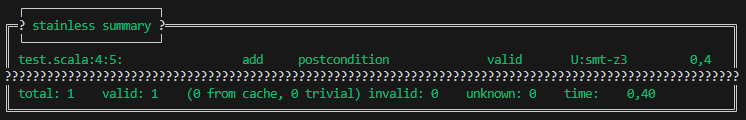
\includegraphics[width=1.1\textwidth]{images/add.png}
  \caption{The summary Stainless provides after verifying the add function in 
  Listing~\ref{lst:add}.}
  \label{fig:add}
\end{figure}


Stainless is however not compatible with all Scala programs.
It only supports a subset of Scala known as Pure Scala.

\subsection{Pure Scala}
\label{sec:pure_scala}


Pure Scala is a purely functional subset of Scala that 
Stainless accepts as input~\cite{StainlessPureScala}. 
Understanding it is directly relevant to this project, 
as it is a key factor in determining which SV-COMP 
Java benchmarks are translatable into programs that Stainless 
can process.

Pure Scala is structured around ADTs (algebraic data types),
programs are built from \texttt{abstract class} hierarchies 
and immutable \texttt{case class} definitions~\cite{StainlessPureScala}. 
Pure Scala does support methods, inheritance, and overriding, 
but restricts classes to immutable fields. However, 
mutable \texttt{var} fields in classes and null references 
are not supported~\cite{KuncakStainlessTutorial}. 
Mutable data structures from the Scala standard library are not supported,
as Pure Scala enforces a functional, side-effect-free
style, which means that functions cannot modify a state 
outside of their own scope~\cite{StainlessPureScala}.

For numeric types, Pure Scala provides \texttt{BigInt} for unbounded
integers with no overflow semantics and \texttt{Int} as a 32-bit
integer with standard overflow semantics. In this project, 
\texttt{BigInt} is preferred over \texttt{Int} when 
translating Java programs that use Java's \texttt{int} type, 
as it avoids overflow cases which complicates the verification process.

Beyond Pure Scala, Stainless also supports an extension
that makes it possible to use \texttt{var} declarations
and \texttt{while} loops~\cite{StainlessImperative}.
Stainless handles them by transforming them into equivalent 
Pure Scala constructs before verification. This is directly relevant
for this project as Java \texttt{for} loops are converted into 
\texttt{while} loops in corresponding translated Scala programs.
\texttt{while} loops can be annotated with loop invariants
which Stainless verifies as holding on each iteration of the loop and
on termination of the loop.  

\section{SV-COMP}
\label{sec:svcomp}

SV-COMP~\cite{SV-COMP} (Competition on Software Verification) is an annual
international competition that compares software verification tools on a
large set of verification tasks.
The most recent edition, SV-COMP 2026, evaluated 61 verifiers and
16 validators for C programs and 11 verifiers and 3 validators for Java
programs~\cite{SV-COMP2026}.
All benchmark programs and their specifications are publicly
available in the \texttt{sv-benchmarks} repository~\cite{SVBenchmarks}, and any researcher may
contribute new tasks which fit the competition's quality
criteria~\cite{SV-COMP}.
 
\subsection{Benchmark Structure}
\label{sec:svcomp-structure}
 
Each verification task in SV-COMP consists of a program to be
verified, properties which the program is expected to satisfy, and an
expected verdict.
The expected verdict is either \texttt{TRUE} if the program is known to
satisfy the property, or \texttt{FALSE} if it is known to violate it.
This expected verdict is used to determine whether a verifier's output is
correct or not.
 
A verifier participating in SV-COMP produces one of the following outcomes
for each task:
 
\begin{itemize}
  \item \texttt{TRUE}, meaning the verifier concludes that the program satisfies
        the properties for all possible executions.
  \item \texttt{FALSE}, meaning the verifier concludes that one or all of the
  properties are violated and typically produces a counterexample.
  \item \texttt{UNKNOWN}, meaning the verifier could not reach a conclusion.
  \item \texttt{Timeout} or \texttt{Out Of Memory}, meaning the verifier exhausted
        its allocated resources without producing a result.
\end{itemize}
 
The scoring of each verifier is determined by the correctness of its results.
Correct results are awarded points, whilst incorrect results are penalised.
A correct \texttt{TRUE} or correct \texttt{FALSE} result earns points,
whereas an incorrect result (a \texttt{TRUE} verdict on a task that has an
expected verdict of \texttt{FALSE}, or vice versa) results in a penalty.
This scoring scheme is intentional, as it is considered worse to
wrongly assert correctness of a buggy program than to %change->%
admit inability to decide.
 
\subsection{Categories}
\label{sec:svcomp-categories}
 
The benchmark tasks are organised into a hierarchy of categories.
At the top level, SV-COMP 2026 has several meta categories for C
programs, including \texttt{C.ReachSafety}, \texttt{C.MemSafety},
\texttt{C.Concurrency}, \texttt{C.NoOverflows}, \texttt{C.Termination},
and \texttt{C.SoftwareSystems}, all accumulated under \texttt{C.Overall}.
There is also a separate meta category for Java programs called
\texttt{Java.Overall}~\cite{SV-COMP2026} which is the focus of the
translation work in this project.
 
The C categories contain the vast majority of tasks. For example, in
the 2026 edition, \texttt{C.Overall} alone contained 36\,402 tasks.
The Java category is considerably smaller, 1\,731 tasks in 2026,
covering two properties for Java programs.

\subsection{Java.Overall}
\label{sec:svcomp-java}

Since this project focuses on translating Java benchmarks to Scala, the
\texttt{Java.Overall} category is the directly relevant part of SV-COMP.
In SV-COMP 2026, it contained two base categories:
\texttt{Java.valid-assert.Main} and \texttt{Java.no-runtime-exception.Main}~\cite{SV-COMP2026}.
 
The \texttt{valid-assert} property requires that all assertions in
the program hold for every possible execution.
In the Java benchmarks, this is encoded directly through
\texttt{assert} statements in the source code. The expected verdict is
\texttt{TRUE} if no assertion can be violated for any possible input, and
\texttt{FALSE} if an execution reaches a failing assertion.
The \texttt{no-runtime-exception} property requires that the Java
program does not throw a runtime exception under any input.
 
The Java benchmarks in the repository are drawn from a range of sources,
including test suites from established Java verification tools such as
\texttt{JayHorn}~\cite{JayHorn} and \texttt{JBMC}~\cite{JBMC}, as well as
programs from algorithmic benchmark suites~\cite{SV-COMP2026}.
This variety means that the tasks range from small programs with a
single algorithmic pattern to more complex programs with 
loops and recursion.
 
\subsection{Benchmark Infrastructure}
\label{sec:svcomp-infra}
 
SV-COMP uses BenchExec~\cite{BenchExec} to execute and measure all
verification runs in a controlled and reproducible way.
BenchExec enforces resource limits on each run. In 2026 these were
15\,GB of memory and 15 minutes of cumulative CPU time on 4 processing
units. BenchExec also precisely measures CPU time and memory usage for each task.
This execution environment ensures that the results of the different tools
and different editions of the competition are comparable.

In this project, Stainless is not run inside the official BenchExec
infrastructure, as integrating Stainless into the SV-COMP toolchain
is beyond the scope of this project.
Instead, the translated benchmarks are run with Stainless directly and
the outcomes are compared against the expected SV-COMP verdicts and the
results reported by Java verifiers in the competition.

\chapter{Methodology}
\label{cha:methodology}

I followed an empirical methodology in
which I treated Stainless as the system under study and its verification
outcomes on adapted SV-COMP benchmarks served as the data. I first
had to choose a subset of the Java benchmarks I was going to evaluate 
following some parameters (see \Cref{sec:benchmark-selection}).
Then, I translated the selected benchmarks to equivalent Scala programs 
suitable for Stainless (see \Cref{sec:benchmark-selection}).
While translating the programs I had to add additional annotations and 
formal specifications to the translated code to make them 
suitable for Stainless (see \Cref{sec:annotation}).
I then ran Stainless on the translated benchmarks under the same 
resource limits as SV-COMP (see \Cref{sec:experimental-setup}) and collected the 
results to then analyze and compare them against the expected
SV-COMP verdicts and the results reported by Java verifiers 
in the competition (see \Cref{sec:data-collection}). 
 
% ============================================================
\section{Benchmark Selection}
\label{sec:benchmark-selection}
% ============================================================
 
The SV-COMP benchmark repository~\cite{SVBenchmarks} contains a large
number of tasks across many categories. As described in
\Cref{sec:svcomp-java}, the \texttt{Java.Overall} category in
SV-COMP~2026 consists of 1\,731 tasks.
Evaluating all of these is outside the scope of this project, so I selected
a subset of them.
 
My primary criterion for inclusion in the subset was \emph{translatability}.
I included a benchmark only if I could translate it into a Pure
Scala program that Stainless can process. I excluded several classes of benchmarks
based on these criteria:
 
\begin{itemize}
  %rewrite a bit%
  \item Benchmarks that rely on Java specific features with no direct
        Scala equivalent.
  \item Benchmarks that depend on external Java libraries or runtime
        behaviour that I could not reproduce inside Stainless's supported
        subset of Scala.
\end{itemize}

\begin{figure}[t]
\begin{lstlisting}[language=Java, basicstyle=\ttfamily\scriptsize]
import org.sosy_lab.sv_benchmarks.Verifier;
import rbtree.RedBlackTree;
import rbtree.RedBlackTreeNode;

public class Main {
  public static void main(String[] args) {
    int N = Verifier.nondetInt();
    Verifier.assume(N > 0);

    try {
      RedBlackTree tree = new RedBlackTree();

      for (int i = 0; i < N; i++) {
        int data = Verifier.nondetInt();
        tree.treeInsert(new RedBlackTreeNode(data));
      }

      int data = Verifier.nondetInt();
      RedBlackTreeNode node = tree.treeSearch(tree.root(), data);
    } catch (Exception e) {
      assert false;
    }
  }
}
\end{lstlisting}
\caption{An excluded benchmark utilizing external packages 
and exception handling.}
\label{fig:excluded-benchmark}
\end{figure}

For example, the \texttt{RedBlackTree} benchmarks from the 
\texttt{algorithms} category were excluded because they rely 
heavily on external package imports
and exception handling, which aren't directly translatable to Stainless's 
Pure Scala subset. \Cref{fig:excluded-benchmark} illustrates this 
untranslatable structure.

Within the remaining translatable benchmarks, I chose a representative subset 
to cover both property types (\texttt{valid-assert} and
\texttt{no-runtime-exception}) and a range of program structures,
including simple programs, programs with loops, and programs
with recursion. This
variety allows my evaluation to identify patterns in what Stainless
handles well and where it encounters difficulties, rather than reporting
a single success rate over a homogeneous workload.
 
%I gave priority to benchmarks drawn from established Java verification
%tool suites such as JayHorn~\cite{JayHorn} and JBMC~\cite{JBMC}, as
%these tend to be well specified and have clear expected verdicts that are
%independently confirmed.
 
% ============================================================
\section{Translation from Java to Scala}
\label{sec:translation}
% ============================================================
 
Since Stainless operates on a functional subset of Scala, the selected
Java benchmarks cannot be passed to Stainless directly. I manually translated each benchmark
from Java to Scala which is supported by Stainless. I performed the translation
manually rather than through an automated tool, because the structural
differences between Java and Stainless's supported subset of Scala require
some judgement. Specifically, I had to decide how to preserve the program's 
semantics while conforming to Pure Scala's restrictions, 
without making any changes to
the original meaning of the program or giving Stainless any unfair 
advantages or disadvantages.

I followed several general principles during the translation process, 
which I describe below.
 
\subsection{Data Types}
\label{sec:translation-types}
 
Java programs primarily use primitive integer types such as \texttt{int}.
In the translated Scala programs, I systematically replaced Java's \texttt{int}
with Stainless's \texttt{BigInt} type, which represents unbounded mathematical
integers and carries no overflow semantics. I made this choice to avoid the
complication of modelling Java's 32 bit or 64 bit wrap around arithmetic,
which would require modular arithmetic and would complicate the verification
process significantly.

An example of this can be seen in the translation of the \texttt{Ackermann}
benchmark, which is shown in \cref{fig:datatype-translation}.

\begin{figure}[htbp]
\begin{minipage}[t]{0.48\textwidth}
\textbf{Original Java (32 bit int):}
\begin{lstlisting}[language=Java, basicstyle=\ttfamily\scriptsize]
public static int ack(int m, int n) {
    if (m == 0) {
      return n + 1;
    }
    if (n == 0) {
      return ack(m - 1, 1);
    }
    return ack(m - 1, ack(m, n - 1));
  }
\end{lstlisting}
\end{minipage}
\hfill
\begin{minipage}[t]{0.48\textwidth}
\textbf{Translated Scala (Unbounded BigInt):}
\begin{lstlisting}[language=Scala, basicstyle=\ttfamily\scriptsize]
def ack(m: BigInt, n: BigInt): BigInt = {
    if (m == 0)
      n + 1
    else if (n == 0)
      ack(m - 1, 1)
    else
      ack(m - 1, ack(m, n - 1))
  }
\end{lstlisting}
\end{minipage}
\caption{Translation of the \texttt{Ackermann} benchmark, demonstrating the conversion from bounded 32-bit integers to unbounded \texttt{BigInt} to avoid overflow semantics.}
\label{fig:datatype-translation}
\end{figure}


\subsection{Control Flow}
\label{sec:translation-control}

I translated Java's \texttt{for} and \texttt{while} loops into Scala
\texttt{while} loops. Stainless allows \texttt{while} loops through its imperative
extension~\cite{StainlessImperative}, and converts them into Pure Scala before
verifying them. I chose to keep the loop structures exactly as they were in Java
to stay faithful to the original benchmarks, rather than rewriting them into
recursive functions (which Stainless usually handles more easily).

 
\subsection{Assertions and Properties}
\label{sec:translation-assertions}
 
Benchmarks in SV-COMP often evaluate both properties simultaneously 
(\texttt{valid-assert} and \texttt{no-runtime-exception}), 
and these properties can sometimes have different expected verdicts 
within the exact same benchmark. 

To verify \texttt{valid-assert} properties, the original Java benchmarks
use \texttt{assert} statements. When translating these to Scala, 
I converted them into Stainless's \texttt{assert} expressions or 
incorporated them directly as function postconditions using 
Stainless's \texttt{ensuring} keyword. Stainless then verifies 
these statically as proof obligations.

On the other hand, for the \texttt{no-runtime-exception} property, no explicit 
annotations or assertions are required. Stainless automatically 
verifies the absence of runtime errors such as array out of bounds 
access and division by zero using its built in verification 
process~\cite{StainlessOriginal}.
 
% ============================================================
\section{Specification and Annotation}
\label{sec:annotation}
% ============================================================
 
A key difference between testing and deductive verification is that
Stainless must be given enough information about a program's intended
behaviour to be able to construct a proof. 
While translating properties into \texttt{assert}
or \texttt{ensuring} expressions is often enough for simple code,
programs with loops or recursion additionally require the user to supply
loop invariants or termination measures.
 
\textbf{Loop invariants:}
A loop invariant is a predicate that must hold at the start of each
iteration and after the loop terminates. For \texttt{while} loops in
the translated benchmarks, I provided loop invariants using Stainless's
\texttt{.invariant()} method attached directly to the loop block. I constructed these 
invariants by analyzing the logic of the original Java loops. Understanding what 
the loop was intended to do, as well as knowing whether the benchmark was expected 
to pass or fail, made it easier to determine what mathematical properties 
needed to be tracked during verification.

\Cref{fig:insertion-sort} shows an example of a translated benchmark with loop invariants.
The original benchmark is \texttt{InsertionSort-FunSat01}.

\begin{figure}[t]
\begin{lstlisting}[language=Scala, basicstyle=\ttfamily\scriptsize]
def sort(a: Array[Int]): Unit = {
  require(a.length >= 0)
  val N = a.length
  var i = 1
  (while (i < N) {
    decreases(N - i)
    var j = i - 1
    var x = a(i)
    (while ((j >= 0) && (a(j) > x)) {
      decreases(j + 1)
      a(j + 1) = a(j)
      j = j - 1
    }).invariant(j >= -1 && j < i && i < N && a.length == N)
    a(j + 1) = x
    i = i + 1
  }).invariant(i >= 1 && i <= N && a.length == N)
}
\end{lstlisting}
\caption{The translated Scala \texttt{sort} method from \texttt{InsertionSort-FunSat01}, showing loop invariants and termination measures attached to nested loops.}
\label{fig:insertion-sort}
\end{figure}

 
\textbf{Termination measures:}
Stainless requires termination proofs for all recursive functions to
ensure that a non-terminating function cannot trivially satisfy any
postcondition~\cite{StainlessOriginal}. For recursive benchmarks,
a termination measure is provided using the \texttt{decreases} clause.
The measure must be an expression that strictly decreases on every
recursive call and is bounded below. \Cref{fig:termination-gcd} shows
an example from the \texttt{SatGcd} benchmark, where the sum \texttt{y1 + y2}
serves as the measure: each recursive call either reduces \texttt{y1} or
\texttt{y2} by the other, so the sum strictly decreases.

\begin{figure}[htbp]
\begin{minipage}[t]{0.48\textwidth}
\textbf{Original Java:}
\begin{lstlisting}[language=Java, basicstyle=\ttfamily\scriptsize]
static int gcd(int y1, int y2) {
  if (y1 <= 0 || y2 <= 0)
    return 0;
  if (y1 == y2)
    return y1;
  if (y1 > y2)
    return gcd(y1 - y2, y2);
  return gcd(y1, y2 - y1);
}
\end{lstlisting}
\end{minipage}
\hfill
\begin{minipage}[t]{0.48\textwidth}
\textbf{Translated Scala:}
\begin{lstlisting}[language=Scala, basicstyle=\ttfamily\scriptsize]
def gcd(y1: BigInt, y2: BigInt): BigInt = {
  decreases(y1 + y2)
  require(y1 > 0 && y2 > 0)
  if (y1 <= 0 || y2 <= 0)
    BigInt(0)
  else if (y1 == y2)
    y1
  else if (y1 > y2)
    gcd(y1 - y2, y2)
  else
    gcd(y1, y2 - y1)
}.ensuring(res => res >= 1)
\end{lstlisting}
\end{minipage}
\caption{Translation of the \texttt{SatGcd} benchmark demonstrating a
non-trivial termination measure: \texttt{decreases(y1 + y2)} decreases
on every recursive call since each call reduces one argument by the other.}
\label{fig:termination-gcd}
\end{figure}
 
\textbf{Preconditions and postconditions:}
For benchmarks where the expected verdict is \texttt{TRUE}, I added a
postcondition using the \texttt{.ensuring()} clause to capture the
property that the program should satisfy. For benchmarks where the
expected verdict is \texttt{FALSE}, the goal is to confirm that Stainless
produces a counterexample. In these cases, the assertion remains in the 
translated program, without strengthening the specification, so that Stainless
can find the counterexample.
 
The amount of annotation required varies across the benchmarks.
Simple programs often require no annotation beyond the
assertion itself, while other benchmarks with loops and complex
logic may require more significant annotation effort.
\Cref{fig:addition-translation} illustrates a fully annotated recursive
benchmark, showing the combination of \texttt{BigInt} types, a
\texttt{decreases} termination measure, and an \texttt{.ensuring}
postcondition in the \texttt{Addition} benchmark.

\begin{figure}[t]
\begin{minipage}[t]{0.48\textwidth}
\textbf{Original Java:}
\begin{lstlisting}[language=Java, basicstyle=\ttfamily\scriptsize]
static int addition(int m, int n) { 
  if (n == 0) {
    return m;
  }
  if (n > 0) {
    return addition(m + 1, n - 1);
  }
  return addition(m - 1, n + 1);
}
\end{lstlisting}
\end{minipage}
\hfill
\begin{minipage}[t]{0.48\textwidth}
\textbf{Translated Scala (with annotations):}
\begin{lstlisting}[language=Scala, basicstyle=\ttfamily\scriptsize]
def addition(m: BigInt, n: BigInt): BigInt = {
  decreases(if (n >= 0) n else -n)
  if(n == 0){
    m
  } else if(n > 0){
    addition(m + 1, n - 1)
  } else {
    addition(m - 1, n + 1)
  }
}.ensuring(res => res == m + n)
\end{lstlisting}
\end{minipage}
\caption{Translation of the \texttt{Addition} benchmark demonstrating \texttt{BigInt} usage, termination measures, and postconditions.}
\label{fig:addition-translation}
\end{figure}


 
% ============================================================
\section{Experimental Setup}
\label{sec:experimental-setup}
% ============================================================
 
I ran all experiments on a single machine with a fixed hardware and
software configuration to ensure that timing measurements are
reproducible. The relevant configuration is as follows.
 
\begin{itemize}
  \item \textbf{Stainless version:} I recorded the version of Stainless used 
        in the artifact alongside the translated benchmarks.
  \item \textbf{SMT solver:} I ran Stainless with its default SMT
        solver configuration, which uses Z3~\cite{Z3} as the primary
        backend.
  \item \textbf{Resource limits:} To replicate the official 
  SV-COMP benchmarking environment as closely as possible, 
  each verification run was constrained to a maximum memory 
  limit of 15 GB of RAM and a time limit of 15 minutes 
  (900 seconds).
\end{itemize}
 
Unlike the official SV-COMP participants, 
who are evaluated using the \texttt{Benchexec} 
framework on Linux machines with strict 
\texttt{cgroups} resource isolation, I conducted 
the experiments for this project locally on a 
Windows machine using a custom batch script since 
\texttt{Benchexec} does not support Windows or WSL. 
% ============================================================
\section{Data Collection and Analysis}
\label{sec:data-collection}
% ============================================================
 
For each translated benchmark, I recorded the following data:
 
\begin{itemize}
  \item The Stainless verdict: \texttt{valid}, \texttt{invalid}
        (with the counterexample if available), \texttt{timeout}, or
        \texttt{unknown}.
  \item The time taken for Stainless to produce the verdict.
  \item The expected SV-COMP verdict (\texttt{TRUE} or \texttt{FALSE}).
  \item Whether the Stainless verdict agrees with the expected verdict.
\end{itemize}
 
The primary measure of success is the \emph{correct verdict rate}, which is the
fraction of benchmarks for which Stainless's verdict matches the expected
SV-COMP verdict. A Stainless \texttt{valid} result is taken to correspond
to a SV-COMP \texttt{TRUE} expected verdict, and a Stainless
\texttt{invalid} result to a \texttt{FALSE} expected verdict.
 
I used the verification results produced by Java verifiers participating in
SV-COMP~2026 as a reference point throughout the analysis.
\chapter{Design}

\chapter{Implementation}

\chapter{Evaluation}

\chapter{Conclusions}

\bibliographystyle{plainurl}
\bibliography{main}

\end{document}

%%% Local Variables: ***
%%% mode: latex ***
%%% TeX-master: "main.tex"  ***
%%% ispell-local-dictionary: "british"  ***
%%% End: ***